\documentclass[portuguese,oneside]{tcc}

\usepackage{graphicx}
\usepackage{multirow}
\usepackage{nicefrac}
\usepackage{algorithmic}
\usepackage{calc}
\usepackage{enumitem}
\usepackage{fixltx2e}

\author{Guilherme de Mello Mattos Taschetto e Pedro Pillon Vanzella}

\title{Inteligência Artificial Aplicada a Elevadores}
      {Artificial Intelligence Applied to Elevators}

\tipotrabalho{\ptci}
\curso{\cc}
\orientador{João Batista de Oliveira}

\begin{document}

\begin{resumo}{elevadores, inteligência artificial, simulação, sistemas multiagentes, aprendizado de máquina}

Elevadores são um meio de transporte utilizado por milhões de pessoas no mundo
inteiro. Com este trabalho, pretende-se propor soluções de Inteligência
Artificial para melhorar a eficiência dos mesmos, reduzindo o tempo que
passageiros despendem em função destes. Através da modelagem e implementação de
um simulador de elevadores e de algoritmos de Inteligência Artificial, espera-se
realizar testes de diferentes técnicas e soluções propostas na literatura, a fim
de propor quais estratégias são mais adequadas para cada cenário.

\end{resumo}

\begin{abstract}{elevators, artificial intelligence, simulation, multiagent systems, machine learning}

Elevators are a mode of transportation used by milions of people around the
world. In this project, we will propose Artificial Intelligence solutions in
order to increase their efficiency, reducing their users' wait times. Through
the process of modeling and implementation of an elevator simulator and
Artificial Intelligence algorithms, we hope to test out the different techniques
and solutions proposed in the literature, in order to propose which strategies
best fit each scenario.

\end{abstract}

\tableofcontents

\chapter{\label{chap:intro}Introdução}

Em 2014, 54\% da população mundial vivia em áreas urbanas, de acordo com a Organização das Nações Unidas~\cite{UN14}. A expectativa é que esta proporção aumente para 66\% até o ano 2050. Em números absolutos isto representa um acréscimo de 2,5 bilhões de pessoas à população urbana mundial nos próximos 35 anos. Uma das consequências da alta densidade populacional em regiões geográficas limitadas é o crescimento do modelo de verticalização na construção civil. Neste cenário, onde prédios de diversos andares se tornam presença no cotidiano da maioria da população, os elevadores passam a um papel de destaque.

Uma pesquisa realizada pela IBM no ano de 2010 em 16 cidades norte-americanas constatou que, durante 12 meses, o tempo acumulado no qual trabalhadores de escritórios\footnote{Em uma força de trabalho total de 51 milhões de trabalhadores, dos quais 12,7 milhões são usuários de elevadores diariamente~\cite{IBM10}.} aguardaram por elevadores foi de 92 anos~\cite{IBM10}. Em uma economia onde o salário horário médio de um trabalhador é de US\$ 24,99, o tempo de espera por elevadores representa custos de mais de US\$ 20 bilhões em média por ano~\cite{BLS15}.

Além do impacto econômico existe o impacto psicológico. Trabalhadores em centros metropolitanos empreendem uma parcela significativa da sua rotina no deslocamento entre residência e local de trabalho e no caminho inverso ao final do dia. Além de gastar uma quantidade significativa de tempo no trânsito das ruas, em carros, ônibus, bicicletas e metrôs, o tempo compreendido entre aguardar o elevador e desembarcar no andar desejado está longe de ser desprezível. Em função disso, ajustam sua rotina abrindo mão de momentos de momentos de descanso ou lazer. Uma possível consequência é um aumento nos níveis de estresse e um decréscimo na qualidade de vida a médio e longo prazo. {\color{red}[BUSCAR FONTES PARA ESTE PARÁGRAFO]} % TODO: CITATIONNEEDED

\begin{figure}[htb!]
\centering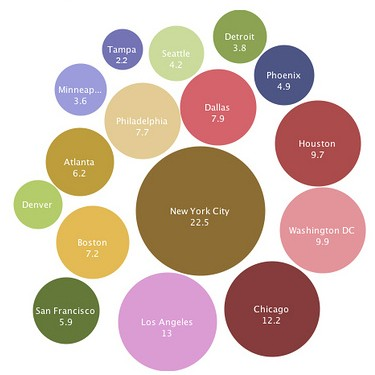
\includegraphics{img/time-cost.jpg}
\caption{\label{fig:fig1}Tempo de espera acumulado (em anos) por elevadores durante 12 meses em 16 cidades norte-americanas. Fonte:~\cite{IBM10}}
\end{figure}

Neste contexto global, a indústria de elevadores possui alguns desafios: primeiro, lidar com a pressão para a redução de custos na construção civil, construindo elevadores mais baratos e eficientes, com melhorias no desempenho de transporte; segundo, competir no mercado oferecendo serviços novos, personalizados e com garantia de qualidade, visando revolucionar a maneira com que elevadores interagem e servem passageiros~\cite{KOEHLEROTTIGER02}. Já sob o ponto de vista dos passageiros, estes esperam que suas chamadas sejam atendidas imediatamente e que sejam levados ao seu destino o mais rápido possível.

Existem diversas abordagens que os fabricantes de elevadores podem usar para minimizar o tempo de espera, como aumentar o número de elevadores no prédio ou a capacidade de cada elevador. Entretanto, este tipo de alteração não é sempre realizável em função de limitações na estrutura do prédio ou inviabilidade financeira. Como alternativa e muitas vezes uma solução de mais fácil aplicação é otimizar o sistema de controle dos elevadores. Ainda assim, a tarefa de atribuir elevadores para atender chamadas minimizando o tempo médio de espera está no conjunto de problemas NP-difícil (ou NP-hard, ou NP-complexo)~\cite{SeKo99}. Portanto, uma solução ótima para este problema ainda não é conhecida.

Desde meados dos anos 1980, a indústria de elevadores vem estudando e implementando estratégias para encontrar soluções sub-ótimas para o problema. Diversas técnicas de Inteligência Artificial foram adotadas, como redes neurais, algoritmos genéticos, lógicas \textit{fuzzy} e, mais recentemente, sistemas multi-agentes, planejamento e aprendizado de máquina~\cite{KOEHLEROTTIGER02}.

A proposta deste trabalho é comparar diferentes estratégias de controle de elevadores em alguns cenários e avaliar, dentre as opções possíveis, quais combinações resultam em um melhor desempenho no transporte de passageiros. A comparação se dará analisando os resultados de simulações de diferentes algoritmos de controle.

Para tanto, serão implementados no mínimo 2 algoritmos para o sistema de controle de elevadores e um simulador de elevadores. O usuário do simulador poderá:

\begin{itemize}
  \item Selecionar cenários;
  \item Selecionar um algoritmo para controle dos elevadores ou implementar o seu próprio;
  \item Comparar o desempenho entre diferentes algoritmos em um mesmo cenário;
  \item Comparar o desempenho de um algoritmo em múltiplos cenários.
\end{itemize}

\section{Métricas de Desempenho de um Sistema de Elevadores}


\begin{description}[leftmargin=!,labelwidth=\widthof{\bfseries HC\textsubscript{5\%}}]
  \item[HC\textsubscript{5\%}]
  Percentual da população total do prédio que um sistema de elevadores consegue transportar em um intervalo de 5 minutos. Um HC\textsubscript{5\%} aceitável é de no mínimo 14\% \cite{KOEHLEROTTIGER02}. Por exemplo, em um prédio cuja população é de 600 pessoas, este índice representa o transporte de no mínimo 84 pessoas em 5 minutos.

  \item[WT]
  \textit{Waiting Time}, ou tempo de espera; está compreendido entre a chegada de um passageiro e o seu embarque em um elevador.

  \item[JT]
  \textit{Journey Time}, ou tempo de jornada; está compreendido entre o embarque de um passageiro em um elevador e o desembarque em seu destino.

  \item[ST]
  \textit{System Time}, ou tempo de sistema; está compreendido entre entre a chegada de um passageiro e o desembarque em seu destino, ou seja, é a soma do tempo de espera com o tempo de jornada.

  \item[AWT]
  \textit{Average Waiting Time}, ou tempo médio de espera.

  \item[AJT]
  \textit{Average Journey Time}, ou tempo médio de jornada.


  \item[AST]
  \textit{Average System Time}, ou tempo médio de sistema.
\end{description}

O tempo médio de sistema define a qualidade do serviço, já que está ligada diretamente à percepção que os passageiros possuem do sistema. É correto afirmar que o desejo de um passageiro é chegar no seu destino o mais rápido possível - ou seja, com o menor tempo de sistema possível. Normalmente, tempos de sistema menores relacionam-se com um alto HC\textsubscript{5\%}; porém, passageiros tendem a dar maior importância a um baixo tempo de espera do que a um baixo tempo de jornada~\cite{KOEHLEROTTIGER02}.

 Ainda assim, embora não seja uma grande melhoria reduzir de 32 para 28 segundos de espera, é psicologicamente importante evitar esperas longas, i. e. 60 segundos ou mais. {\color{red}[BUSCAR FONTES PARA ESTA AFIRMAÇÃO]} % TODO: CITATIONNEEDED

 Assim sendo, o escopo deste trabalho será limitado na busca pela otimização do tempo médio de espera (\textbf{AWT}).

\section{Parâmetros de Definição de Cenários}

\begin{description}[leftmargin=!,labelwidth=\widthof{\bfseries AAA}]
  \item[F]
  Número total de andares do prédio.
  \item[E]
  Número total de elevadores que compõem o sistema.
  \item[K]
  Capacidade máxima de passageiros que um elevador é capaz de transportar.
  \item[P]
  População total do prédio.
  \item[F]
  Função de distribuição de chegada de passageiros.
\end{description}

\section{Glossário}

Termos chaves usados neste trabalho.

\begin{description}[leftmargin=!,labelwidth=\widthof{\bfseries Sistema de Controle}]
  \item[Lobby]                Andar térreo de um prédio.
  \item[Elevador]             Dispositivo de transporte vertical que movimenta pessoas ou cargas entre andares ou níveis de um prédio ou estrutura.
  \item[Sistema de Controle]  O sistema central que gerencia todos os elevadores.
\end{description}
\chapter{\label{chap:problem}Descrição do Problema}

A maior parte dos prédios possui instalações de grupos com 2 a 8 elevadores \cite{KOEHLEROTTIGER02}. Em muitos prédios, esses são o meio de transporte primário entre andares, visto que escadas são menos práticas e, muitas vezes, menos acessíveis ou exclusivas para situações de emergência. Dado o seu uso em larga escala, a ineficiência dos sistemas de controle de elevadores é sentida diariamente por seus usuários. Neste cenário, deseja-se encontrar formas de otimizar estes sistemas de controle de modo a refletir positivamente no desempenho geral do sistema e na percepção da qualidade do sistema na visão de seus usuários.

O problema estudado neste trabalho é modelado da seguinte forma: seja um prédio com \textbf{N} andares e \textbf{M} elevadores, cada um com capacidade para transportar \textbf{K} pessoas simultaneamente; sabe-se que a população total do prédio é \textbf{P} e está distribuída de maneira uniforme nos andares do prédio; também sabe-se que a chegada ou saídas destas pessoas obedece uma função de distribuição de probabilidade \textbf{F}. De que forma o sistema pode atender esta população de modo a minimizar o tempo médio de atendimento de cada pessoa?

\section{Sistema de Controle de Grupo de Elevadores}

Um \textit{Elevator Group Control System} (\textbf{EGCS}), ou sistema de controle de grupo de elevadores, é responsável por coordenar as ações dos elevadores do prédio~\cite{kuzunuki1984elevator}. Esta coordenação visa atender à todas \textbf{chamadas de corredor}\footnote{Passageiros estão fora dos elevadores e realizam uma chamada para subir ou descer à partir do andar em que se encontram.} e \textbf{chamadas de cabine}\footnote{Passageiros estão dentro do elevador e realizam uma chamada para desembarcar em um andar destino.} em um dado instante. O \textbf{estado} do sistema pode ser modelado, minimamente, pelo seguinte conjunto de informações:

\begin{itemize}
  \item Para cada andar:
  \begin{itemize}
    \item Se existe uma \textbf{chamada de corredor} a partir deste andar, o horário em que foi originada e o sentido (subir, descer ou ambos);
  \end{itemize}
  \item Para cada elevador:
  \begin{itemize}
    \item Um conjunto de \textbf{chamadas de cabine} solicitadas pelos passageiros e o horário em que cada uma foi originada;
    \item O andar em que se encontra;
    \item Se está parado, subindo ou descendo;
    \item Sua lotação.
  \end{itemize}
\end{itemize}

Sobre estes dados, o EGCS utiliza-se de algoritmos e técnicas para fornecer como saída:

\begin{itemize}
  \item Para cada elevador:
  \begin{itemize}
    \item Uma \textbf{sequência de paradas} que aquele elevador deve realizar.
  \end{itemize}
\end{itemize}

Existem eventos após os quais o EGCS deve recalcular as sequências de paradas dos elevadores de modo a atender as novas solicitações. Tais eventos são:

\begin{itemize}
  \item Uma nova \textbf{chamada de corredor};
  \item Uma nova \textbf{chamada de cabine};
  \item Uma \textbf{parada realizada} com alteração significativa na lotação do elevador;
  \item Um elevador torna-se ocioso, i. e., não possuir mais paradas a realizar.
\end{itemize}

\section{Aquisição de Dados e Métricas}

A aquisição de dados sobre o tráfego de um sistema de elevadores instalados é um problema em aberto na indústria~\cite{KOEHLEROTTIGER02}. Em casos simples é possível designar pessoas para observar e contar passageiros entrando e saindo dos elevadores. Já em casos mais complexos foram aplicadas soluções mais engenhosas, como contagem de pessoas aplicando algoritmos de visão computacional em vídeos de câmeras de segurança e sensores de carga. Estas abordagens possuem fatores complicadores - como, por exemplo, a dificuldade em lidar com as diferenças de iluminação, baixa qualidade de vídeo, baixa precisão de sensores, etc - e o resultado obtido não compensa o custo.

A simulação de sistemas de elevadores ganha destaque neste contexto, tornando-se uma alternativa atraente para obter métricas e avaliar o desempenho de um sistema na fase de projeto, antes da sua construção. Algumas das principais métricas utilizadas pela indústria de elevadores para avaliar o desempenho de seus sistemas são:

\begin{description}[leftmargin=!,labelwidth=\widthof{\bfseries HC\textsubscript{5\%}}]
  \item[HC\textsubscript{5\%}]
  Percentual da população total do prédio que um sistema de elevadores consegue transportar em um intervalo de 5 minutos. Um HC\textsubscript{5\%} aceitável é de no mínimo 14\%~\cite{KOEHLEROTTIGER02}. Por exemplo, em um prédio cuja população é de 600 pessoas, este índice representa o transporte de no mínimo 84 pessoas em 5 minutos.

  \item[WT]
  \textit{Waiting Time}, ou tempo de espera; está compreendido entre a requisição de um passageiro e o seu embarque em um elevador.

  \item[JT]
  \textit{Journey Time}, ou tempo de jornada; está compreendido entre o embarque de um passageiro em um elevador e o desembarque em seu destino.

  \item[ST]
  \textit{System Time}, ou tempo de sistema; está compreendido entre entre a chegada de um passageiro e o desembarque em seu destino, ou seja, é a soma do tempo de espera com o tempo de jornada.

  \item[AWT]
  \textit{Average Waiting Time}, ou tempo médio de espera.

  \item[AJT]
  \textit{Average Journey Time}, ou tempo médio de jornada.

  \item[AST]
  \textit{Average System Time}, ou tempo médio de sistema.

  \item[RTT]
  \textit{Round-trip Time}, ou tempo de ida e volta em uma tradução livre; é o tempo médio de uma viagem de um elevador partindo do lobby, indo até todos os andares do prédio e de volta ao lobby em horário de pico.
\end{description}

O tempo médio de sistema (AST) define a qualidade do serviço, já que está ligado diretamente à percepção que os passageiros possuem do sistema. É correto afirmar que o desejo de um passageiro é chegar no seu destino o mais rápido possível - ou seja, com o menor tempo de sistema possível. Normalmente, tempos de sistema menores relacionam-se com um alto HC\textsubscript{5\%}; porém, passageiros tendem a dar maior importância a um baixo tempo de espera do que a um baixo tempo de jornada~\cite{KOEHLEROTTIGER02}. Isto por que, uma vez dentro do elevador, o passageiro não se sente mais esperando: ele sente que já está sendo servido.

{\color{red}Ainda assim, embora uma redução de 32 para 28 segundos de espera não seja considerada uma grande melhoria, é psicologicamente importante evitar esperas longas, i.~e.~60 segundos ou mais.} % TODO: CITATIONNEEDED

\section{Padrões de Comportamento}

Há três padrões principais que descrevem o comportamento de grupos de
passageiros em relação aos elevadores.

\begin{description}[leftmargin=!,labelwidth=\widthof{\bfseries interfloor}]
  \item[up peak]    Passageiros chegam no lobby e desejam subir.
  \item[down peak]  Passageiros desejam descer de qualquer andar para o lobby.
  \item[interfloor] Passageiros deslocam-se entre andares arbitrários, com exceção do lobby.
\end{description}

Outros padrões podem ser definidos combinando-se os três padrões acima
descritos. No entanto, para os fins deste trabalho, nos limitaremos aos padrões puros.

\section{Cenários}

Pode-se dizer que cada prédio é um cenário em potencial no contexto deste trabalho. Alguns dos principais atributos que podem ser utilizados para definir um cenário são:

\begin{description}[leftmargin=!,labelwidth=\widthof{\bfseries Propósito}]
  \item[N]
  Número total de andares do prédio.
  \item[M]
  Número total de elevadores que compõem o sistema.
  \item[K]
  Capacidade\footnote{Como efeito de redução de escopo consideraremos todos os
    elevadores de um mesmo sistema como tendo a mesma capacidade.} (em número de
  pessoas\footnote{Consideramos uma pessoa com peso médio de 70kg.}) máxima de passageiros que cada elevador é capaz de transportar.
  \item[P]
  População total do prédio.
  \item[F]
  Função de distribuição de probabilidade de chegada/saída de passageiros.
  \item[Propósito]
  Propósito do prédio: residencial, comercial com múltiplas empresas, comercial com única empresa, etc;
\end{description}

Logo, há tantos cenários possíveis quanto há prédios ao redor do mundo.
Entretanto, por limitação de tempo e de recursos computacionais, vamos limitar
os cenários em algumas categorias. A escolha destas divisões é arbitrária, com
fim didático, exceto pelo limite inferior de 4 andares devido à exigência legal
do Município de Porto Alegre onde prédios deste tamanho ou maiores (mas não
menores que isto) de serem construídos com elevadores. O limite
superior\footnote{O maior arranha-céu do mundo em 2015 é o Burj Khalif,
  localizado em Dubai, com mais de 800m de altura, em 160 andares habitáveis.} fica em aberto.

% \footnote{http://www2.portoalegre.rs.gov.br/cgi-bin/nph-brs?u=/netahtml/sirel/avancada.html&p=3&r=59&f=G&d=ATOS&l=20&s1=(ELEVADOR)..RELA. }

\begin{table}[htb!]
\centering
\caption{Cenários}
\label{table:tab1}
\begin{tabular}{|l|c|c|c|c|}
\hline
{\bf Cenário}        & {\bf N}    & {\bf M} & {\bf K} & {\bf P} \\ \hline
{\it Prédio pequeno} & 4 a 5      & 1       & 6       & 40      \\ \hline
{\it Prédio médio}   & 6 a 10     & 2       & 10      & 96      \\ \hline
{\it Pŕedio grande}  & 11 a 30    & 5       & 10      & 560     \\ \hline
{\it Arranha-céu}    & 30 ou mais & 10      & 12      & 3200    \\ \hline
\end{tabular}
\end{table}

{\color{red}[SERIA BEM MELHOR SE USÁSSEMOS DADOS REAIS PARA MKP DE PRÉDIOS CONHECIDOS. EX: PŔEDIO ONDE MORAMOS, FACIN, EMPIRE STATE, BURJ KHALIF, ETC]} % TODO

\section{Critérios de Aceitação}

Uma tecnologia que saiba endereçar as seguintes questões será de grande interesse para a indústria de elevadores~\cite{KOEHLEROTTIGER02}:

\begin{enumerate}
\item Qual é a função objetivo de um algoritmo de despache em grupo? \hfill \newline
      Almost no information is published by companies about the objective functions they use in their con- trol algorithms. Usually, a vague “combination of waiting and journey times” is minimized, but which function would yield the best possi- ble results still seems to be an open question.

\item Como um sistema de controle pode obter informações adicionais acerca das necessidades dos passageiros?\hfill \newline
      In particular, how can it find out how many passengers are waiting at a floor, how fully loaded a car is, and where the passengers want to go?

\item Como o desempenho do controlador pode ser melhorado? \hfill \newline
      Is it possible to detect and predict patterns of traffic based on the cur- rently available information and/or previously learned patterns? How could such information be exploited by a control algorithm?

\item De quê forma as interfaces com os passageiros podem evoluir além de simples botões? \hfill \newline
      How can passengers with special needs be better served? In the following, we give an overview of AI- based approaches that have been explored by elevator companies in the past to address these issues.
\end{enumerate}

\section{Possíveis Complicadores}

Um número de cenários pode complicar as métricas e prejudicar os resultados. A grande maioria destes complicadores são fatores humanos, como pessoas segurando a porta, passageiros indecisos, seleção acidental de andares e desistências após chamar o elevador.

Alguns destes problemas podem ser mitigados com a modificação da interface dos elevadores. Por exemplo, seleções acidentais de andares poderiam ser desfeitas, caso houvesse um mecanismo para cancelar a seleção de um andar. O mesmo vale para o cenário do passageiro indeciso.

No entanto, propor este tipo de alteração de comportamento não está no escopo deste trabalho. É nosso objetivo estudar alterações somente nos algoritmos que regem o comportamento dos elevadores da maneira com que estão atualmente instalados na vasta maioria dos prédios.
\chapter{\label{chap:proposal}Proposta do Trabalho}

A proposta deste trabalho será estudar métodos de inteligência artificial,
aplicados a elevadores, de modo a aumentar a eficiência de grupos de elevadores.

As conseqüências imediatas esperadas deste aumento de eficiência são um ganho de
qualidade de vida para os potenciais passageiros, bem como um aumento de
produtividade de alguns grupos dos mesmos.

MODELAGEM

AGENTES

FUNÇÃO-OBJETIVO
\chapter{\label{chap:stages}Etapas do Trabalho}

\begin{itemize}
    \item Estudar o funcionamento de elevadores e possibilidades de comportamento
    \item Estudar métodos de inteligência artificial utilizados em elevadores
    \item Definir cenários de testes
    \item Modelar o simulador
    \item Implementar algoritmos de IA
    \item Realizar simulações
    \item Comparar resultados obtidos
\end{itemize}

\section{Cronograma}

O cronograma do trabalho será dividido em \textit{sprints} de duas semanas. 

\subsection{TCC 1}
\subsubsection{Sprint 1}
\subsubsection{Sprint 2}

\subsection{TCC 2}
\chapter{\label{chap:related}Trabalhos Relacionados}

Alguns trabalhos já abordaram a temática de Inteligência Artificial aplicada a
elevadores. O artigo ``\textit{An AI-based approac to destination control in
  elevators}''~\cite{KOEHLEROTTIGER02} descreve o problema e o classifica como
NP-Hard.  %TODO CONTINUAR




\section{Destination Dispatch}

%http://www.schindler.com/br/internet/pt/solucoes-em-mobilidade/produtos/gerenciamento-acesso/miconic-10.html

Rockefeller Center, New York NY
Prime Tower, Zurich, Switzerland (2011)

%http://www.schindler.com/br/internet/pt/solucoes-em-mobilidade/produtos/gerenciamento-acesso/port-technology.html

EZ Towers
São Paulo, 2012

Doha Twin Towers
Doha, 2013

%https://www.thyssenkruppelevator.com/elevator-products/elevator-destination-dispatch#tab1

World Financial Center, NY, EUA

\section{Double-deck Elevators}

%http://www.schindler.com/content/au/internet/en/mobility-solutions/products/elevators/schindler-7000/_jcr_content/rightPar/downloadlist_0/downloadList/16_1336648631250.download.asset.16_1336648631250/DD_Brochure.pdf

Utilizado em:

Burj Khalifa in Dubai
Petronas Twin Towers in Kuala Lumpur
Statue of Liberty in New York (goes no higher than the pedestal)

\section{Two elevators, same shaft}

https://twin.thyssenkrupp-elevator.com/

Utilizado em:

European Central Bank, Frankfurt, Alemanha
ThyssenKrupp Headquarters, Essen, Alemanha
Mercury Tower Lot 14, Moscou, Russie
\chapter{\label{chap:conclusion}Conclusão}

Com elevadores presentes na vida de tantos habitantes de grandes centros
urbanos, eles são um alvo óbvio para otimização.

Como vimos anteriormente, algumas tentativas de utilização de Inteligência
Artificial aplicadas aos mesmos foram feitas. Entende-se que um simulador que
permita a avaliação objetiva e comparação de diferentes estratégias em
diferentes cenários será de grande valor, permitindo que decisões a respeito da
otimização e melhoria deste meio de transporte sejam tomadas.

A análise cuidadosa dos dados estatísticos gerados por este simulador permitirá
que uma estratégia vantajosa seja encontrada para cada cenário.

\bibliographystyle{tcc-num}
\bibliography{bib-proposta}

\end{document}
